% Created by tikzDevice version 0.12.6 on 2026-08-12 08:13:51
% !TEX encoding = UTF-8 Unicode
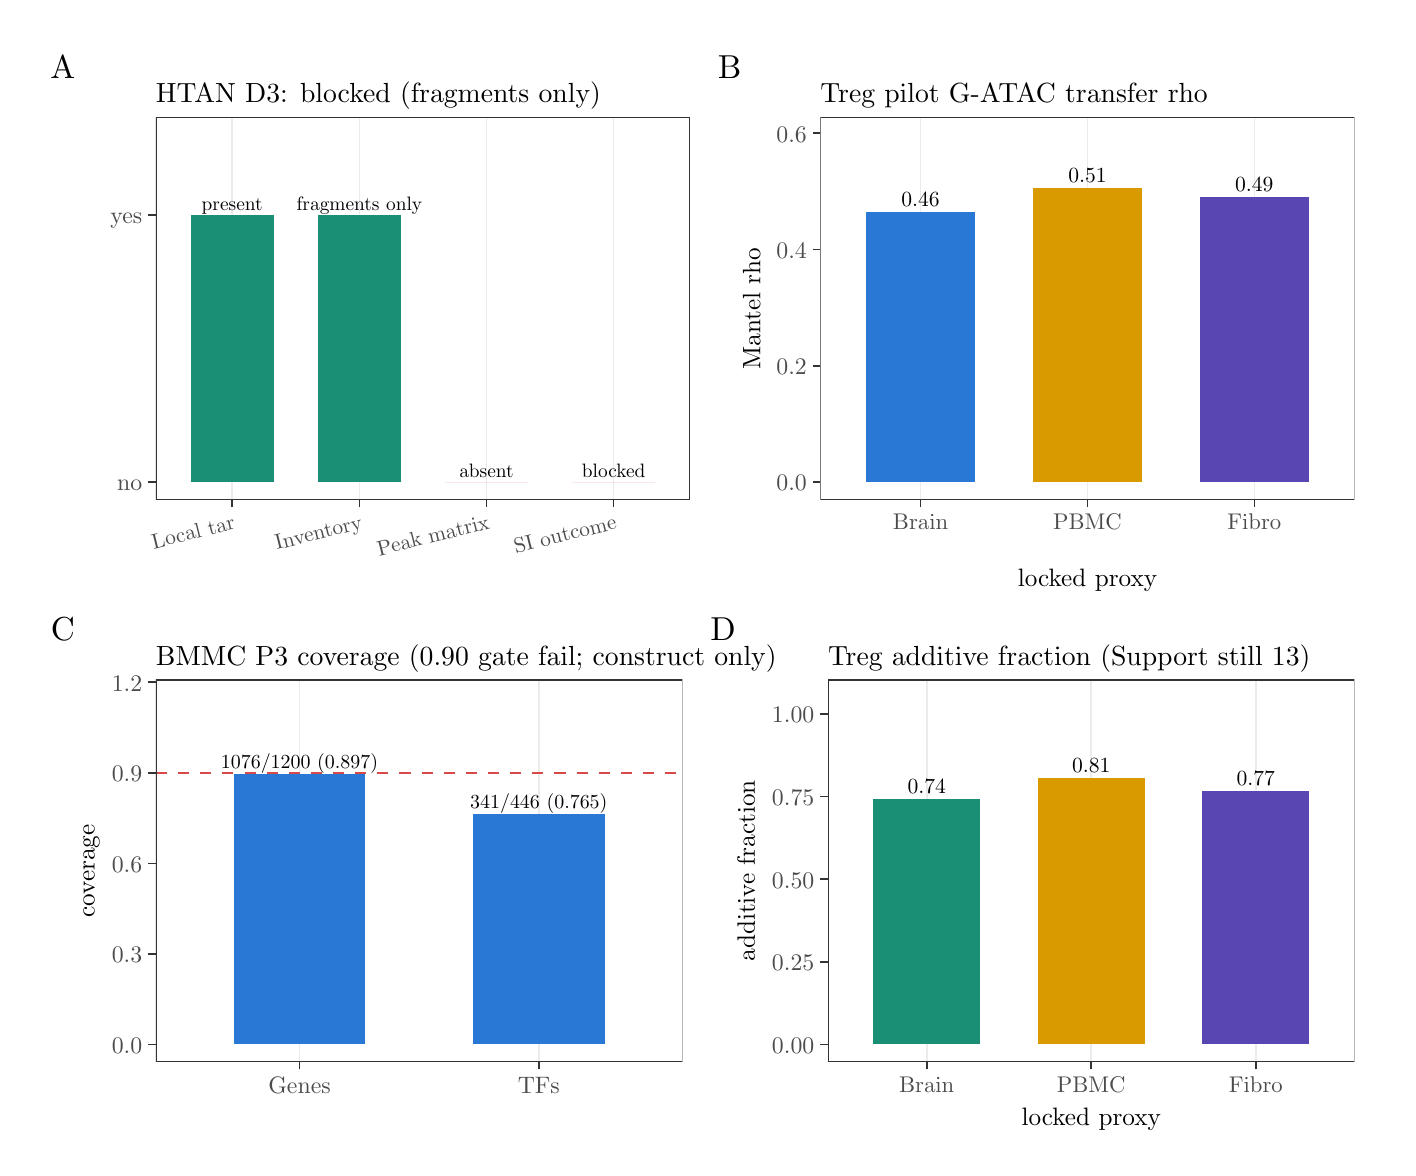
\begin{tikzpicture}[x=1pt,y=1pt]
\definecolor{fillColor}{RGB}{255,255,255}
\path[use as bounding box,fill=fillColor,fill opacity=0.00] (0,0) rectangle (491.44,404.71);
\begin{scope}
\path[clip] (  0.00,  0.00) rectangle (491.44,404.71);
\definecolor{drawColor}{RGB}{255,255,255}
\definecolor{fillColor}{RGB}{255,255,255}

\path[draw=drawColor,line width= 0.6pt,line join=round,line cap=round,fill=fillColor] ( -0.00, -0.00) rectangle (491.44,404.71);
\end{scope}
\begin{scope}
\path[clip] (  4.00,197.50) rectangle (245.31,400.71);
\definecolor{drawColor}{RGB}{255,255,255}
\definecolor{fillColor}{RGB}{255,255,255}

\path[draw=drawColor,line width= 0.6pt,line join=round,line cap=round,fill=fillColor] (  4.00,197.50) rectangle (245.31,400.71);
\end{scope}
\begin{scope}
\path[clip] (245.31,197.50) rectangle (485.44,400.71);
\definecolor{drawColor}{RGB}{255,255,255}
\definecolor{fillColor}{RGB}{255,255,255}

\path[draw=drawColor,line width= 0.6pt,line join=round,line cap=round,fill=fillColor] (245.31,197.50) rectangle (485.44,400.71);
\end{scope}
\begin{scope}
\path[clip] ( 46.35,234.24) rectangle (239.31,372.21);
\definecolor{fillColor}{RGB}{255,255,255}

\path[fill=fillColor] ( 46.35,234.24) rectangle (239.31,372.21);
\definecolor{drawColor}{gray}{0.92}

\path[draw=drawColor,line width= 0.6pt,line join=round] ( 73.91,234.24) --
	( 73.91,372.21);

\path[draw=drawColor,line width= 0.6pt,line join=round] (119.85,234.24) --
	(119.85,372.21);

\path[draw=drawColor,line width= 0.6pt,line join=round] (165.80,234.24) --
	(165.80,372.21);

\path[draw=drawColor,line width= 0.6pt,line join=round] (211.74,234.24) --
	(211.74,372.21);
\definecolor{fillColor}{RGB}{27,143,117}

\path[fill=fillColor] ( 58.98,240.51) rectangle ( 88.84,336.99);

\path[fill=fillColor] (104.92,240.51) rectangle (134.79,336.99);
\definecolor{fillColor}{RGB}{216,74,74}

\path[fill=fillColor] (150.87,240.51) rectangle (180.73,240.51);

\path[fill=fillColor] (196.81,240.51) rectangle (226.67,240.51);
\definecolor{drawColor}{RGB}{0,0,0}

\node[text=drawColor,anchor=base,inner sep=0pt, outer sep=0pt, scale=  0.70] at ( 73.91,338.55) {present};

\node[text=drawColor,anchor=base,inner sep=0pt, outer sep=0pt, scale=  0.70] at (119.85,338.55) {fragments only};

\node[text=drawColor,anchor=base,inner sep=0pt, outer sep=0pt, scale=  0.70] at (165.80,242.06) {absent};

\node[text=drawColor,anchor=base,inner sep=0pt, outer sep=0pt, scale=  0.70] at (211.74,242.06) {blocked};
\definecolor{drawColor}{gray}{0.20}

\path[draw=drawColor,line width= 0.6pt,line join=round,line cap=round] ( 46.35,234.24) rectangle (239.31,372.21);
\end{scope}
\begin{scope}
\path[clip] (  0.00,  0.00) rectangle (491.44,404.71);
\definecolor{drawColor}{gray}{0.30}

\node[text=drawColor,anchor=base east,inner sep=0pt, outer sep=0pt, scale=  0.86] at ( 41.40,237.31) {no};

\node[text=drawColor,anchor=base east,inner sep=0pt, outer sep=0pt, scale=  0.86] at ( 41.40,333.80) {yes};
\end{scope}
\begin{scope}
\path[clip] (  0.00,  0.00) rectangle (491.44,404.71);
\definecolor{drawColor}{gray}{0.20}

\path[draw=drawColor,line width= 0.6pt,line join=round] ( 43.60,240.51) --
	( 46.35,240.51);

\path[draw=drawColor,line width= 0.6pt,line join=round] ( 43.60,336.99) --
	( 46.35,336.99);
\end{scope}
\begin{scope}
\path[clip] (  0.00,  0.00) rectangle (491.44,404.71);
\definecolor{drawColor}{gray}{0.20}

\path[draw=drawColor,line width= 0.6pt,line join=round] ( 73.91,231.49) --
	( 73.91,234.24);

\path[draw=drawColor,line width= 0.6pt,line join=round] (119.85,231.49) --
	(119.85,234.24);

\path[draw=drawColor,line width= 0.6pt,line join=round] (165.80,231.49) --
	(165.80,234.24);

\path[draw=drawColor,line width= 0.6pt,line join=round] (211.74,231.49) --
	(211.74,234.24);
\end{scope}
\begin{scope}
\path[clip] (  0.00,  0.00) rectangle (491.44,404.71);
\definecolor{drawColor}{gray}{0.30}

\node[text=drawColor,rotate= 14.00,anchor=base east,inner sep=0pt, outer sep=0pt, scale=  0.77] at ( 75.30,223.74) {Local tar};

\node[text=drawColor,rotate= 14.00,anchor=base east,inner sep=0pt, outer sep=0pt, scale=  0.77] at (121.24,223.74) {Inventory};

\node[text=drawColor,rotate= 14.00,anchor=base east,inner sep=0pt, outer sep=0pt, scale=  0.77] at (167.18,223.74) {Peak matrix};

\node[text=drawColor,rotate= 14.00,anchor=base east,inner sep=0pt, outer sep=0pt, scale=  0.77] at (213.12,223.74) {SI outcome};
\end{scope}
\begin{scope}
\path[clip] (  0.00,  0.00) rectangle (491.44,404.71);
\definecolor{drawColor}{RGB}{0,0,0}

\node[text=drawColor,anchor=base west,inner sep=0pt, outer sep=0pt, scale=  1.00] at ( 46.35,377.58) {HTAN D3: blocked (fragments only)};
\end{scope}
\begin{scope}
\path[clip] (  0.00,  0.00) rectangle (491.44,404.71);
\definecolor{drawColor}{RGB}{0,0,0}

\node[text=drawColor,anchor=base,inner sep=0pt, outer sep=0pt, scale=  1.20] at ( 12.74,386.41) {A};
\end{scope}
\begin{scope}
\path[clip] (286.48,234.24) rectangle (479.44,372.21);
\definecolor{fillColor}{RGB}{255,255,255}

\path[fill=fillColor] (286.48,234.24) rectangle (479.44,372.21);
\definecolor{drawColor}{gray}{0.92}

\path[draw=drawColor,line width= 0.6pt,line join=round] (322.66,234.24) --
	(322.66,372.21);

\path[draw=drawColor,line width= 0.6pt,line join=round] (382.96,234.24) --
	(382.96,372.21);

\path[draw=drawColor,line width= 0.6pt,line join=round] (443.26,234.24) --
	(443.26,372.21);
\definecolor{fillColor}{RGB}{42,120,214}

\path[fill=fillColor] (303.06,240.51) rectangle (342.25,338.08);
\definecolor{fillColor}{RGB}{217,154,0}

\path[fill=fillColor] (363.36,240.51) rectangle (402.55,346.81);
\definecolor{fillColor}{RGB}{89,70,178}

\path[fill=fillColor] (423.66,240.51) rectangle (462.85,343.42);
\definecolor{drawColor}{RGB}{0,0,0}

\node[text=drawColor,anchor=base,inner sep=0pt, outer sep=0pt, scale=  0.78] at (322.66,340.09) {0.46};

\node[text=drawColor,anchor=base,inner sep=0pt, outer sep=0pt, scale=  0.78] at (382.96,348.82) {0.51};

\node[text=drawColor,anchor=base,inner sep=0pt, outer sep=0pt, scale=  0.78] at (443.26,345.43) {0.49};
\definecolor{drawColor}{gray}{0.20}

\path[draw=drawColor,line width= 0.6pt,line join=round,line cap=round] (286.48,234.24) rectangle (479.44,372.21);
\end{scope}
\begin{scope}
\path[clip] (  0.00,  0.00) rectangle (491.44,404.71);
\definecolor{drawColor}{gray}{0.30}

\node[text=drawColor,anchor=base east,inner sep=0pt, outer sep=0pt, scale=  0.86] at (281.53,237.31) {0.0};

\node[text=drawColor,anchor=base east,inner sep=0pt, outer sep=0pt, scale=  0.86] at (281.53,279.33) {0.2};

\node[text=drawColor,anchor=base east,inner sep=0pt, outer sep=0pt, scale=  0.86] at (281.53,321.34) {0.4};

\node[text=drawColor,anchor=base east,inner sep=0pt, outer sep=0pt, scale=  0.86] at (281.53,363.36) {0.6};
\end{scope}
\begin{scope}
\path[clip] (  0.00,  0.00) rectangle (491.44,404.71);
\definecolor{drawColor}{gray}{0.20}

\path[draw=drawColor,line width= 0.6pt,line join=round] (283.73,240.51) --
	(286.48,240.51);

\path[draw=drawColor,line width= 0.6pt,line join=round] (283.73,282.52) --
	(286.48,282.52);

\path[draw=drawColor,line width= 0.6pt,line join=round] (283.73,324.54) --
	(286.48,324.54);

\path[draw=drawColor,line width= 0.6pt,line join=round] (283.73,366.55) --
	(286.48,366.55);
\end{scope}
\begin{scope}
\path[clip] (  0.00,  0.00) rectangle (491.44,404.71);
\definecolor{drawColor}{gray}{0.20}

\path[draw=drawColor,line width= 0.6pt,line join=round] (322.66,231.49) --
	(322.66,234.24);

\path[draw=drawColor,line width= 0.6pt,line join=round] (382.96,231.49) --
	(382.96,234.24);

\path[draw=drawColor,line width= 0.6pt,line join=round] (443.26,231.49) --
	(443.26,234.24);
\end{scope}
\begin{scope}
\path[clip] (  0.00,  0.00) rectangle (491.44,404.71);
\definecolor{drawColor}{gray}{0.30}

\node[text=drawColor,anchor=base,inner sep=0pt, outer sep=0pt, scale=  0.82] at (322.66,223.23) {Brain};

\node[text=drawColor,anchor=base,inner sep=0pt, outer sep=0pt, scale=  0.82] at (382.96,223.23) {PBMC};

\node[text=drawColor,anchor=base,inner sep=0pt, outer sep=0pt, scale=  0.82] at (443.26,223.23) {Fibro};
\end{scope}
\begin{scope}
\path[clip] (  0.00,  0.00) rectangle (491.44,404.71);
\definecolor{drawColor}{RGB}{0,0,0}

\node[text=drawColor,anchor=base,inner sep=0pt, outer sep=0pt, scale=  0.91] at (382.96,202.65) {locked proxy};
\end{scope}
\begin{scope}
\path[clip] (  0.00,  0.00) rectangle (491.44,404.71);
\definecolor{drawColor}{RGB}{0,0,0}

\node[text=drawColor,rotate= 90.00,anchor=base,inner sep=0pt, outer sep=0pt, scale=  0.91] at (264.80,303.22) {Mantel rho};
\end{scope}
\begin{scope}
\path[clip] (  0.00,  0.00) rectangle (491.44,404.71);
\definecolor{drawColor}{RGB}{0,0,0}

\node[text=drawColor,anchor=base west,inner sep=0pt, outer sep=0pt, scale=  1.00] at (286.48,377.58) {Treg pilot G-ATAC transfer rho};
\end{scope}
\begin{scope}
\path[clip] (  0.00,  0.00) rectangle (491.44,404.71);
\definecolor{drawColor}{RGB}{0,0,0}

\node[text=drawColor,anchor=base,inner sep=0pt, outer sep=0pt, scale=  1.20] at (253.69,386.41) {B};
\end{scope}
\begin{scope}
\path[clip] (  4.00,  3.00) rectangle (242.58,197.50);
\definecolor{drawColor}{RGB}{255,255,255}
\definecolor{fillColor}{RGB}{255,255,255}

\path[draw=drawColor,line width= 0.6pt,line join=round,line cap=round,fill=fillColor] (  4.00,  3.00) rectangle (242.58,197.50);
\end{scope}
\begin{scope}
\path[clip] (242.58,  3.00) rectangle (485.44,197.50);
\definecolor{drawColor}{RGB}{255,255,255}
\definecolor{fillColor}{RGB}{255,255,255}

\path[draw=drawColor,line width= 0.6pt,line join=round,line cap=round,fill=fillColor] (242.58,  3.00) rectangle (485.44,197.50);
\end{scope}
\begin{scope}
\path[clip] ( 46.35, 31.02) rectangle (236.58,169.00);
\definecolor{fillColor}{RGB}{255,255,255}

\path[fill=fillColor] ( 46.35, 31.02) rectangle (236.58,169.00);
\definecolor{drawColor}{gray}{0.92}

\path[draw=drawColor,line width= 0.6pt,line join=round] ( 98.23, 31.02) --
	( 98.23,169.00);

\path[draw=drawColor,line width= 0.6pt,line join=round] (184.70, 31.02) --
	(184.70,169.00);
\definecolor{fillColor}{RGB}{42,120,214}

\path[fill=fillColor] ( 74.45, 37.30) rectangle (122.01,135.10);

\path[fill=fillColor] (160.92, 37.30) rectangle (208.48,120.69);
\definecolor{drawColor}{RGB}{216,74,74}

\path[draw=drawColor,line width= 0.8pt,dash pattern=on 4pt off 4pt ,line join=round] ( 46.35,135.46) -- (236.58,135.46);
\definecolor{drawColor}{RGB}{0,0,0}

\node[text=drawColor,anchor=base,inner sep=0pt, outer sep=0pt, scale=  0.72] at ( 98.23,136.98) {1076/1200 (0.897)};

\node[text=drawColor,anchor=base,inner sep=0pt, outer sep=0pt, scale=  0.72] at (184.70,122.57) {341/446 (0.765)};
\definecolor{drawColor}{gray}{0.20}

\path[draw=drawColor,line width= 0.6pt,line join=round,line cap=round] ( 46.35, 31.02) rectangle (236.58,169.00);
\end{scope}
\begin{scope}
\path[clip] (  0.00,  0.00) rectangle (491.44,404.71);
\definecolor{drawColor}{gray}{0.30}

\node[text=drawColor,anchor=base east,inner sep=0pt, outer sep=0pt, scale=  0.86] at ( 41.40, 34.10) {0.0};

\node[text=drawColor,anchor=base east,inner sep=0pt, outer sep=0pt, scale=  0.86] at ( 41.40, 66.82) {0.3};

\node[text=drawColor,anchor=base east,inner sep=0pt, outer sep=0pt, scale=  0.86] at ( 41.40, 99.54) {0.6};

\node[text=drawColor,anchor=base east,inner sep=0pt, outer sep=0pt, scale=  0.86] at ( 41.40,132.26) {0.9};

\node[text=drawColor,anchor=base east,inner sep=0pt, outer sep=0pt, scale=  0.86] at ( 41.40,164.99) {1.2};
\end{scope}
\begin{scope}
\path[clip] (  0.00,  0.00) rectangle (491.44,404.71);
\definecolor{drawColor}{gray}{0.20}

\path[draw=drawColor,line width= 0.6pt,line join=round] ( 43.60, 37.30) --
	( 46.35, 37.30);

\path[draw=drawColor,line width= 0.6pt,line join=round] ( 43.60, 70.02) --
	( 46.35, 70.02);

\path[draw=drawColor,line width= 0.6pt,line join=round] ( 43.60,102.74) --
	( 46.35,102.74);

\path[draw=drawColor,line width= 0.6pt,line join=round] ( 43.60,135.46) --
	( 46.35,135.46);

\path[draw=drawColor,line width= 0.6pt,line join=round] ( 43.60,168.18) --
	( 46.35,168.18);
\end{scope}
\begin{scope}
\path[clip] (  0.00,  0.00) rectangle (491.44,404.71);
\definecolor{drawColor}{gray}{0.20}

\path[draw=drawColor,line width= 0.6pt,line join=round] ( 98.23, 28.27) --
	( 98.23, 31.02);

\path[draw=drawColor,line width= 0.6pt,line join=round] (184.70, 28.27) --
	(184.70, 31.02);
\end{scope}
\begin{scope}
\path[clip] (  0.00,  0.00) rectangle (491.44,404.71);
\definecolor{drawColor}{gray}{0.30}

\node[text=drawColor,anchor=base,inner sep=0pt, outer sep=0pt, scale=  0.86] at ( 98.23, 19.68) {Genes};

\node[text=drawColor,anchor=base,inner sep=0pt, outer sep=0pt, scale=  0.86] at (184.70, 19.68) {TFs};
\end{scope}
\begin{scope}
\path[clip] (  0.00,  0.00) rectangle (491.44,404.71);
\definecolor{drawColor}{RGB}{0,0,0}

\node[text=drawColor,rotate= 90.00,anchor=base,inner sep=0pt, outer sep=0pt, scale=  0.91] at ( 24.22,100.01) {coverage};
\end{scope}
\begin{scope}
\path[clip] (  0.00,  0.00) rectangle (491.44,404.71);
\definecolor{drawColor}{RGB}{0,0,0}

\node[text=drawColor,anchor=base west,inner sep=0pt, outer sep=0pt, scale=  1.00] at ( 46.35,174.37) {BMMC P3 coverage (0.90 gate fail; construct only)};
\end{scope}
\begin{scope}
\path[clip] (  0.00,  0.00) rectangle (491.44,404.71);
\definecolor{drawColor}{RGB}{0,0,0}

\node[text=drawColor,anchor=base,inner sep=0pt, outer sep=0pt, scale=  1.20] at ( 12.74,183.19) {C};
\end{scope}
\begin{scope}
\path[clip] (289.20, 31.02) rectangle (479.44,169.00);
\definecolor{fillColor}{RGB}{255,255,255}

\path[fill=fillColor] (289.20, 31.02) rectangle (479.44,169.00);
\definecolor{drawColor}{gray}{0.92}

\path[draw=drawColor,line width= 0.6pt,line join=round] (324.87, 31.02) --
	(324.87,169.00);

\path[draw=drawColor,line width= 0.6pt,line join=round] (384.32, 31.02) --
	(384.32,169.00);

\path[draw=drawColor,line width= 0.6pt,line join=round] (443.77, 31.02) --
	(443.77,169.00);
\definecolor{fillColor}{RGB}{27,143,117}

\path[fill=fillColor] (305.55, 37.30) rectangle (344.19,125.92);
\definecolor{fillColor}{RGB}{217,154,0}

\path[fill=fillColor] (365.00, 37.30) rectangle (403.64,133.46);
\definecolor{fillColor}{RGB}{89,70,178}

\path[fill=fillColor] (424.45, 37.30) rectangle (463.09,128.79);
\definecolor{drawColor}{RGB}{0,0,0}

\node[text=drawColor,anchor=base,inner sep=0pt, outer sep=0pt, scale=  0.78] at (324.87,127.93) {0.74};

\node[text=drawColor,anchor=base,inner sep=0pt, outer sep=0pt, scale=  0.78] at (384.32,135.47) {0.81};

\node[text=drawColor,anchor=base,inner sep=0pt, outer sep=0pt, scale=  0.78] at (443.77,130.80) {0.77};
\definecolor{drawColor}{gray}{0.20}

\path[draw=drawColor,line width= 0.6pt,line join=round,line cap=round] (289.20, 31.02) rectangle (479.44,169.00);
\end{scope}
\begin{scope}
\path[clip] (  0.00,  0.00) rectangle (491.44,404.71);
\definecolor{drawColor}{gray}{0.30}

\node[text=drawColor,anchor=base east,inner sep=0pt, outer sep=0pt, scale=  0.86] at (284.25, 34.10) {0.00};

\node[text=drawColor,anchor=base east,inner sep=0pt, outer sep=0pt, scale=  0.86] at (284.25, 63.96) {0.25};

\node[text=drawColor,anchor=base east,inner sep=0pt, outer sep=0pt, scale=  0.86] at (284.25, 93.83) {0.50};

\node[text=drawColor,anchor=base east,inner sep=0pt, outer sep=0pt, scale=  0.86] at (284.25,123.69) {0.75};

\node[text=drawColor,anchor=base east,inner sep=0pt, outer sep=0pt, scale=  0.86] at (284.25,153.56) {1.00};
\end{scope}
\begin{scope}
\path[clip] (  0.00,  0.00) rectangle (491.44,404.71);
\definecolor{drawColor}{gray}{0.20}

\path[draw=drawColor,line width= 0.6pt,line join=round] (286.45, 37.30) --
	(289.20, 37.30);

\path[draw=drawColor,line width= 0.6pt,line join=round] (286.45, 67.16) --
	(289.20, 67.16);

\path[draw=drawColor,line width= 0.6pt,line join=round] (286.45, 97.03) --
	(289.20, 97.03);

\path[draw=drawColor,line width= 0.6pt,line join=round] (286.45,126.89) --
	(289.20,126.89);

\path[draw=drawColor,line width= 0.6pt,line join=round] (286.45,156.75) --
	(289.20,156.75);
\end{scope}
\begin{scope}
\path[clip] (  0.00,  0.00) rectangle (491.44,404.71);
\definecolor{drawColor}{gray}{0.20}

\path[draw=drawColor,line width= 0.6pt,line join=round] (324.87, 28.27) --
	(324.87, 31.02);

\path[draw=drawColor,line width= 0.6pt,line join=round] (384.32, 28.27) --
	(384.32, 31.02);

\path[draw=drawColor,line width= 0.6pt,line join=round] (443.77, 28.27) --
	(443.77, 31.02);
\end{scope}
\begin{scope}
\path[clip] (  0.00,  0.00) rectangle (491.44,404.71);
\definecolor{drawColor}{gray}{0.30}

\node[text=drawColor,anchor=base,inner sep=0pt, outer sep=0pt, scale=  0.82] at (324.87, 20.02) {Brain};

\node[text=drawColor,anchor=base,inner sep=0pt, outer sep=0pt, scale=  0.82] at (384.32, 20.02) {PBMC};

\node[text=drawColor,anchor=base,inner sep=0pt, outer sep=0pt, scale=  0.82] at (443.77, 20.02) {Fibro};
\end{scope}
\begin{scope}
\path[clip] (  0.00,  0.00) rectangle (491.44,404.71);
\definecolor{drawColor}{RGB}{0,0,0}

\node[text=drawColor,anchor=base,inner sep=0pt, outer sep=0pt, scale=  0.91] at (384.32,  8.16) {locked proxy};
\end{scope}
\begin{scope}
\path[clip] (  0.00,  0.00) rectangle (491.44,404.71);
\definecolor{drawColor}{RGB}{0,0,0}

\node[text=drawColor,rotate= 90.00,anchor=base,inner sep=0pt, outer sep=0pt, scale=  0.91] at (262.80,100.01) {additive fraction};
\end{scope}
\begin{scope}
\path[clip] (  0.00,  0.00) rectangle (491.44,404.71);
\definecolor{drawColor}{RGB}{0,0,0}

\node[text=drawColor,anchor=base west,inner sep=0pt, outer sep=0pt, scale=  1.00] at (289.20,174.37) {Treg additive fraction (Support still 13)};
\end{scope}
\begin{scope}
\path[clip] (  0.00,  0.00) rectangle (491.44,404.71);
\definecolor{drawColor}{RGB}{0,0,0}

\node[text=drawColor,anchor=base,inner sep=0pt, outer sep=0pt, scale=  1.20] at (251.32,183.19) {D};
\end{scope}
\end{tikzpicture}
